\chapter{Entity Relation Analysis}
	\section{Introduction}
	After the requirements have been set. We need to translate them into workable relational entities in order to be able to modeled through a classical
	relational database system (RDBMS).
	\section{Entities}
	We will start our exploration by defining our entities for this project.
	\subsection{Scan}
	A scan is the result of an ultrasound scan performed in a specific patient(see [\ref{patient-definition})]. A scan entity has certain attributes
	\begin{center}
		\begin{tabular}{ |c|c| } 
			\hline
			Image & The image produced by the ultrasound scan. 360x560 pixels\\
			Prediction & The result of the prediction algorithm. Acceptable Values = {Maligrant, Benign}  \\
			Results & The logs of the algorithm performed the prediction, Optional \\
			Algorithm & The algorithm used to perform the prediction. Acceptable Values = {SVC,RES} \\
			Token& The scan identifier across the application services. token type is UUID [\cite{rfc4122}] \\
			\hline
		\end{tabular}
	\end{center}
	\subsection{Patient}
	\label{patient-definition}
	A patient is a physical person that is suspected to have a thuroid nodule. A person may have 0 up to n scans, where n is the theoretical
	maximum number of records(no limit is enforced by the database or the application). A patient has characteristics explaned below
	\begin{center}
		\begin{tabular}{ |c|c| } 
			\hline
			First Name & The first name of the patient.\\
			Last Name & The last name of the patient \\
			NiNo & The National Insurance Number(NiNo) of the patient \\
			Enrolled Date & The Date that the patient was registered in the system \\
			Ascosiate Doctor& The Doctor identification number, handling the case of the patient(see \ref{doctor-definition}) \\
			Comments& The Doctors(see \ref{doctor-definition}) comments for the particular patient\\
			\hline
		\end{tabular}
	\end{center}
	\subsection{Doctor}
	\label{doctor-definition}
	A doctor is a physical person with access on the system. Is the end-user of the system and has rights of uploading ultrasound image
	scans and retrieve predictions for those scans. It can also provide feedback to the system for a given prediction to be used for 
	further research and develepoment. A doctor has specific characteristics presented below.
	\begin{center}
		\begin{tabular}{ |c|c| } 
			\hline
			Username & Plain-text username\\
			Password & MD5 Hashed[\cite{rfc1321}] and salted[\cite{MANBER1996171}] password \\
			First Name & National Insurance Number[\cite{nino-format}] \\
			Last Name & The date that the patient was registered in the system \\
			Title& The title of the doctor.\\
			Enrolled Date& The date and time of the user enrolled to the system\\
			Last Seen& The date and time of last login of the user \\
			Online Status& The status of the user, acceptable values are Connected,Not Connected \\
			Tasks& The number of scans uploaded by the user \\
			\hline
		\end{tabular}
	\end{center}
	\subsection{Notification}
	\label{notification-definition}
	A notification is a short message from the system to the end-user(The doctor). Its sole purpose is to inform the user about
	various events that may interest the end-user. An example of this may be that the scan results for a given scan task are ready 
	to view. A notification has specific characteristics witch are displayed and explained below.
	\begin{center}
		\begin{tabular}{ |c|c| } 
			\hline
			Message & The message in question\\
			Ascosiated Doctor & The receipient doctor identification number \\
			Created Date & The Date and Time where the event in question where happened\\
			\hline
		\end{tabular}
	\end{center}
	\section{Entity Relations}
	The aforementioned entities have well defined relations. An exhaustive list is given below
	\begin{itemize}
		\item A doctor has many patients (1 - $\infty$)
		\item A doctor has many notifications(1 - $\infty$)
		\item A Patient has many Scans(1 - $\infty$)
	\end{itemize}
	A above relations can be summarized in the following E-R\footnote{Entity-Relation} Diagram
	\begin{figure}[H]
		\iftrue
		\centering
		\caption{Entity-Relation Diagram}
		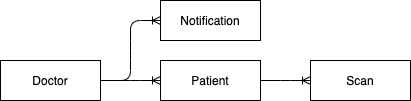
\includegraphics[scale=0.5]{figures/Entity-Relation-Fig}
		\fi
	\end{figure}


